\documentclass{beamer}

\usepackage[francais]{babel}
\usepackage[T1]{fontenc}
\usepackage[latin1]{inputenc}
\usepackage{soul}

\usetheme{Boadilla}
\setbeamertemplate{footline}[frame number,logo]
\usenavigationsymbolstemplate{}

\title{DICOM}
\subtitle{Cours HEdS Gen\`eve}
\author[B. Deville]{Beno\^it Deville - Analyste en informatique}
\institute[HUG]{H\^opitaux Universitaires de Gen\`eve}
\date{Novembre 2015}

\begin{document}

\frame{\titlepage}

% outline
\section*{Plan}
\frame
{
  \frametitle{Plan}
  \tableofcontents
}

% repeat outline at each section
\AtBeginSection[] % Do nothing for \section*
{
      \begin{frame}<beamer>
         \frametitle{Rappel du plan}
         \tableofcontents[currentsection]
      \end{frame}
}

\section{Notions pr\'eliminaires}

	\frame
	{
		\frametitle{Qu'est-ce que DICOM ?}
		
		\begin{block}{\textbf{D}igital \textbf{I}maging and \textbf{Co}mmunications in \textbf{M}edicine}
			\begin{itemize}
				\item< 2-> Digital = Num\'erique
		    		\item<2-> Imaging = Imagerie
		    		\item<3-> Communications
		    		\item<4-> Medicine
			\end{itemize}
		\end{block}

		\begin{itemize}
			\item<5-> Plus de $7400$ pages r\'eparties en $20$ chapitres.
			\item<6-> Documentation compl\`ete gratuite et disponible sur le site d\'edi\'e : \url{https://www.dicomstandard.org/current}	
		\end{itemize}
	}


\section{Histoire du DICOM}

	\frame
	{
		\frametitle{Pourquoi DICOM ?}
		
		\begin{itemize}
			\item<1-> Arriv\'ee du num\'erique en m\'edecine.
			\item<2-> Stockage, transmission, affichage des images : constructeur d\'ependant.
			\item<3-> Solutions propri\'etaires (par opposition \`a solutions ouvertes) :
			\begin{itemize}
				\item<4-> argument commercial : "Mon protocole est meilleur que les autres", "Nos produits ont une excellente interaction entre eux", "Nous g\'erons tout de A \`a Z" ;
				\item<5-> interaction impossible entre marques diff\'erentes.
			\end{itemize} 
		\end{itemize} 
	}
					
	\frame
	{
		\frametitle{D\'ebuts du DICOM}
		\includegraphics<1>[width=\linewidth]{./figures/chrono-dicom-1.png}
		\includegraphics<2>[width=\linewidth]{./figures/chrono-dicom-2.png}
		\includegraphics<3>[width=\linewidth]{./figures/chrono-dicom-3.png}
		\includegraphics<4>[width=\linewidth]{./figures/chrono-dicom-4.png}
		%\includegraphics<5>[width=\linewidth]{./figures/chrono-dicom-5.png}
		%\includegraphics<6>[width=\linewidth]{./figures/chrono-dicom-6.png}
		%\includegraphics<7>[width=\linewidth]{./figures/chrono-dicom-7.png}
		%\includegraphics<8>[width=\linewidth]{./figures/chrono-dicom-8.png}
		%\includegraphics<9>[width=\linewidth]{./figures/chrono-dicom-9.png}
		%\includegraphics<10>[width=\linewidth]{./figures/chrono-dicom-10.png}
		%\includegraphics<11>[width=\linewidth]{./figures/chrono-dicom-11.png}
		%\includegraphics<12>[width=\linewidth]{./figures/chrono-dicom-12.png}
		%\includegraphics<13>[width=\linewidth]{./figures/chrono-dicom-13.png}
		%\includegraphics<14>[width=\linewidth]{./figures/chrono-dicom-14.png}
		%\includegraphics<15>[width=\linewidth]{./figures/chrono-dicom-15.png}
		\includegraphics<5>[width=\linewidth]{./figures/chrono-dicom.png}

		\begin{itemize}
			\item<2-> 1\up{\`ere} version ACR/NEMA 300 en 1985 : peu accept\'e car vague et contenant des incoh\'erences.
			\item<3-> 2\up{\`eme} version en 1988 : transmission des images par le connecteur mat\'eriel EIA-485, adopt\'e par quelques constructeurs.

		        \includegraphics<3>[width=.15\linewidth]{./figures/eia-485.png}
			\item<4-> 3\up{\`eme} version en 1993 : support TCP (protocole Internet), donc ind\'ependance du connecteur physique.
		\end{itemize}
	}
	
	\frame
	{
		\frametitle{DICOM aujourd'hui}
		\begin{itemize}
			\item<1-> Norme reconnue mondialement.
			\item<2-> Actuellement en version $2022$d : on nomme d\'esormais les versions selon la p\'eriode de publication (officiellement, toujours en version 3, ou PS3).
			\item<3-> Diversit\'e des \'equipements support\'es : RX, CT, IRM, US, PET, SPECT, Angio, ECG, BT, \ldots
			\item<4-> Adopt\'ee par de nombreux constructeurs : GE, Siemens, Philips, Toshiba, Hologic, \ldots
		\end{itemize}
	}

\section{Principes de DICOM}

	\frame
	{
		\frametitle{Objectifs}
		\begin{itemize}
			\item Trouver un langage commun pour l'\'echange de donn\'ees entre \'equipements d'imagerie m\'edicale.
			\item<2-> Pousser les constructeurs \`a utiliser ce langage commun.
			\item<3-> Standardiser :
			\begin{itemize}
				\item<4-> le stockage (i.e. format de fichier) ;
				\item<5-> et la communication des donn\'ees (i.e. protocoles de communication).
			\end{itemize}
			\item<6-> Offrir des services de base \`a toute nouvelle connexion, sans changement d'un quelconque composant logiciel (\emph{i.e.~Plug~\&~Play}) :
    			\begin{itemize}
        				\item<7-> connexion \`a un syst\`eme d'archivage d'images, \`a une liste de travail ;
        				\item<8-> r\'ecup\'eration / affichage d'images d'autres fournisseurs ;
        				\item<9-> production d'images lisibles par tout syst\`eme respectant la norme.
        			\end{itemize}

		\end{itemize}
	}
	
	\frame
	{
		\frametitle{Prescription d'un examen radiologique}
		\begin{itemize}
			\item Sch\'ematisation de la proc\'edure :
			%\includegraphics<2->[width=\linewidth]{./figures/scenario-1.png}
			%\includegraphics<3->[width=\linewidth]{./figures/scenario-2.png}
			%\includegraphics<4->[width=\linewidth]{./figures/scenario-3.png}
			%\includegraphics<5->[width=\linewidth]{./figures/scenario-4.png}
			%\includegraphics<6->[width=\linewidth]{./figures/scenario-5.png}
			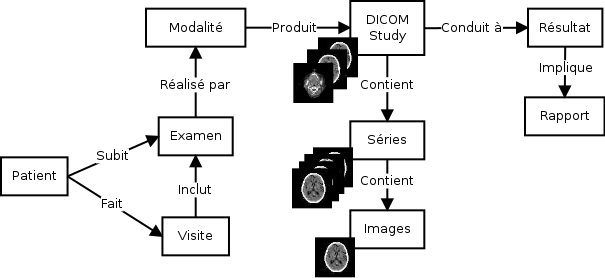
\includegraphics[width=\linewidth]{./figures/scenario.png}
			\item<2-> Donn\'ees et relations d\'ecrites par la norme DICOM (et IHE).
			\item<3-> Le contexte d'utilisation (\emph{e.g.} RIS, PACS, \ldots) d\'etermine le p\'erim\`etre \`a d\'efinir.
		\end{itemize}
	}

	\frame
	{
		\frametitle{Traduire le r\'eel en num\'erique}
		
		\begin{itemize}
			\item Un objet DICOM combine :
			\begin{itemize}
				\item<2-> des donn\'ees, ou \emph{informations} (e.g. un patient, une image, \ldots)
				\begin{itemize}
					\item<3-> contenues dans un \emph{Information Object},
					\item<4-> d\'efini dans la norme par une \emph{Information Object Definition} (ou \emph{IOD}) ;
				\end{itemize}
				
				\item<5-> et une fonction pr\'ecise (e.g. stocker, imprimer,\ldots)
				\begin{itemize}
					\item<6-> c'est-\`a-dire un \emph{Service},
					\item<7-> d\'efini par un \emph{DICOM Message Service Element} (ou \emph{DIMSE})
				\end{itemize}
			\end{itemize}
			\item<8-> Une norme doit lister toutes les combinaisons possibles.
		\end{itemize}
	}
	
	\frame
	{
		\frametitle{Un identifiant unique : le SOP Class UID}

		\begin{itemize}
			\item La combinaison Information Object + Service est :
			\begin{itemize}
				\item<2-> appel\'ee \emph{Service/Object Pair} (ou \emph{SOP}) ;
				\item<3-> un \'el\'ement important pour d\'eterminer la conformit\'e \ la norme ;
				\item<4-> identifi\'ee par un identifiant unique nomm\'e \emph{SOP Class UID}.
			\end{itemize}
		
			\item<5-> Norme DICOM = annuaire de SOP.\\
			SOP Class UID (identifiant unique d'un type de paire service/objet) = num\'ero unique pour trouver \`a quelle paire Service/Objet correspond un objet.
			\item<6-> Analogie : annuaire\\
			Un num\' ero = paire \{nom $+$ adresse\}.
			\item<7-> Exemples de SOP Class UID :
			\begin{description}
				\item<8->[$1.2.840.10008.5.1.4.1.1.1$] CR Image Store (stocker une image de radiologie conventionnelle) ;
				\item<9->[$1.2.840.10008.5.1.4.1.1.2$] CT Image Store (stocker une image CT).
			\end{description}
		\end{itemize}
	}
	
	\frame
	{
		\frametitle{Sch\'ema de construction du SOP}
		\begin{center}
			\includegraphics<1>[width=\linewidth]{./figures/sop-definition.png}
			\includegraphics<2>[width=\linewidth]{./figures/sop-definition-IOD.png}
		\end{center}		
	}


\section{Objets DICOM}

\frame
{
 	\frametitle{Information Object Definition}
  	L'IOD d\'efinit, pour un IO sp\'ecifique, quels sont les attributs qu'on doit/peut trouver dans l'objet.
  	\begin{description}
    		\item<2->[Normalized IOD]~\\
			Repr\'esente une entit\'e unique du monde r\'eel (patient, visite, examen, r\'esultat, interpr\'etation,\ldots)
			
			Complexe et peu performant.
    		\item<3->[Composite IOD]~\\
			Repr\'esente certains d\'etails de plusieurs objets du monde r\'eel, et les relations entre ces objets (nom du patient, date de l'examen,\ldots)
		\item<4->[Attributes]~\\
			Les attributs d'un IOD sont les propri\'et\'es d'un \'el\'ement du monde r\'eel.
  	\end{description}
}

\frame
{
 	\frametitle{IOD composite}
	\includegraphics<2>[width=\linewidth]{./figures/IO-composite-0.png}
	\includegraphics<4>[width=\linewidth]{./figures/IO-composite-1.png}
	\includegraphics<6>[width=\linewidth]{./figures/IO-composite-2.png}
	\includegraphics<8>[width=\linewidth]{./figures/IO-composite-3.png}
	\includegraphics<10>[width=\linewidth]{./figures/IO-composite-4.png}
	\includegraphics<12>[width=\linewidth]{./figures/IO-composite-5.png}
	\includegraphics<14>[width=\linewidth]{./figures/IO-composite-6.png}
	\includegraphics<16>[width=\linewidth]{./figures/IO-composite-7.png}
	\includegraphics<18>[width=\linewidth]{./figures/IO-composite-8.png}
	\includegraphics<20>[width=\linewidth]{./figures/IO-composite.png}
 	\begin{itemize}
		\item<1,3,5,7,9,11,13,15,17,19,21> IOD : agr\'egat d'\emph{Information Entities} ou \emph{IE}.
   		\item<3,5,7,9,11,13,15,17,19,21> Une IE contient un ou plusieurs \emph{Modules}.
		\begin{description}
			\item<5,7,9,11,13,15,17,19,21>[Mandatory] Module obligatoire.
			\item<7,9,11,13,15,17,19,21>[Conditional] Module conditionnel (obligatoire selon certaines conditions).
			\item<9,11,13,15,17,19,21>[User Option] Module optionnel.
		\end{description}
   		\item<11,13,15,17,19,21> Les modules sont compos\'es d'\emph{Attributs} (= valeurs).
		\begin{description}
			\item<13,15,17,19,21>[1] Obligatoire.
			\item<15,17,19,21>[2] Obligatoire - peut \^etre vide.
			\item<17,19,21>[3] Optionnel.
			\item<19,21>[<1/2>C] Conditionnel.
		\end{description}
 	\end{itemize}

	\begin{alertblock}{En pratique}<21>
		Un objet DICOM est presque toujours une instance d'un IOD composite.
	\end{alertblock}
}

\frame
{
 	\frametitle{IOD composite}
	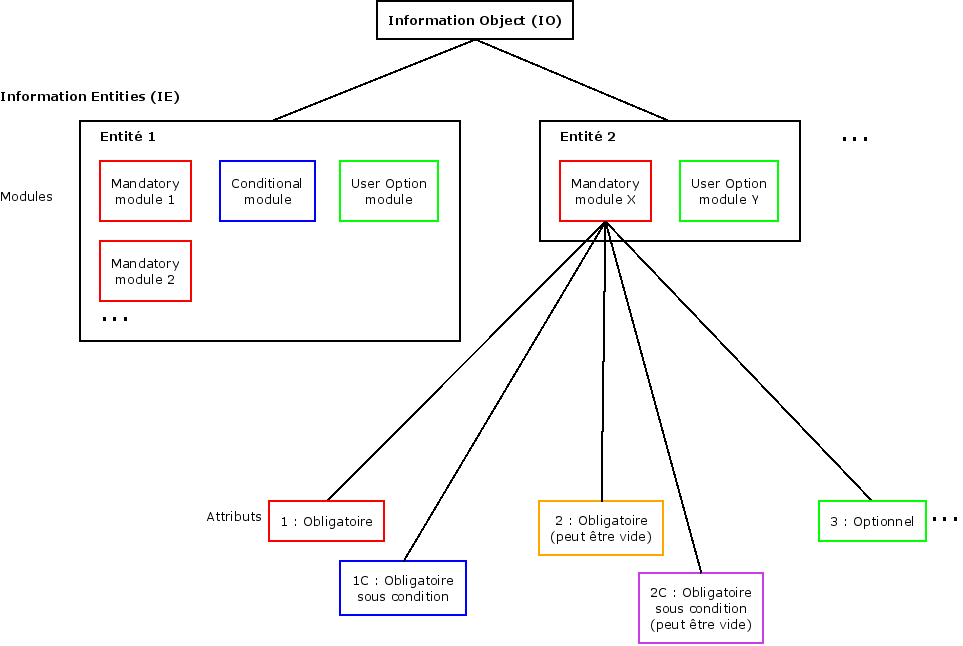
\includegraphics[width=\linewidth]{./figures/IO-composite.png}
}

\frame
{
	\frametitle{Exemple d'IOD : DICOM SR}
	\url{http://dicom.nema.org/medical/dicom/current/output/chtml/part03/sect_A.35.3.3.html}
	\begin{center}
		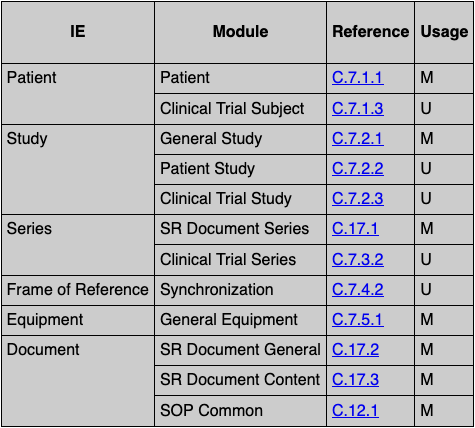
\includegraphics[width=0.5\linewidth]{./figures/IOD-exemple-SR.png}
	\end{center}
}

\frame
{
	\frametitle{Exemple d'IOD : image CR}
	\url{http://dicom.nema.org/medical/dicom/current/output/chtml/part03/sect_A.2.3.html}
	\begin{center}
		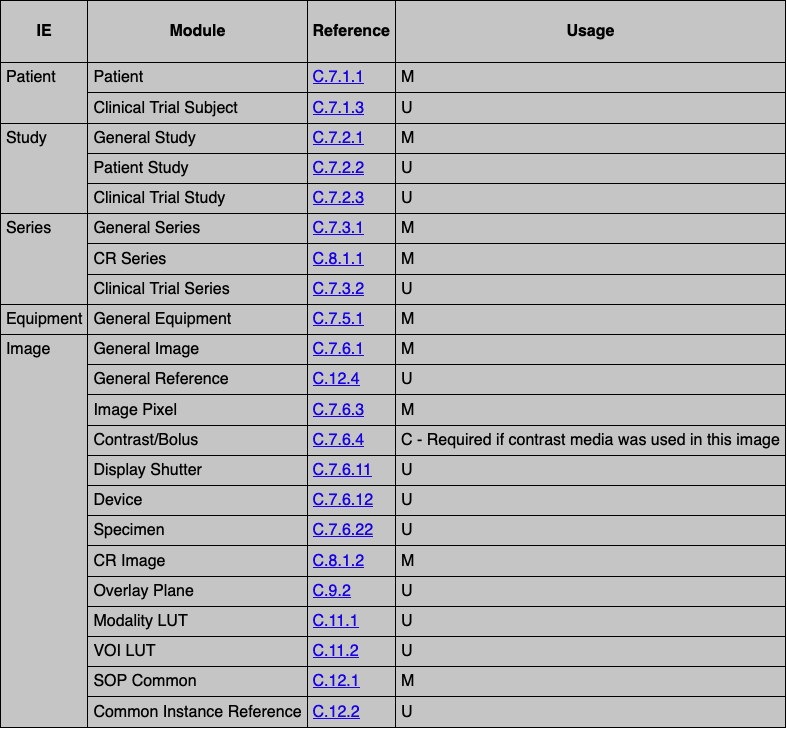
\includegraphics[width=0.6\linewidth]{./figures/IOD-exemple-CR.png}
	\end{center}
}

\frame
{
	\frametitle{Sch\'ema de l'IOD image CR}
	\label{imageCR-IOD}
	
	\begin{center}
		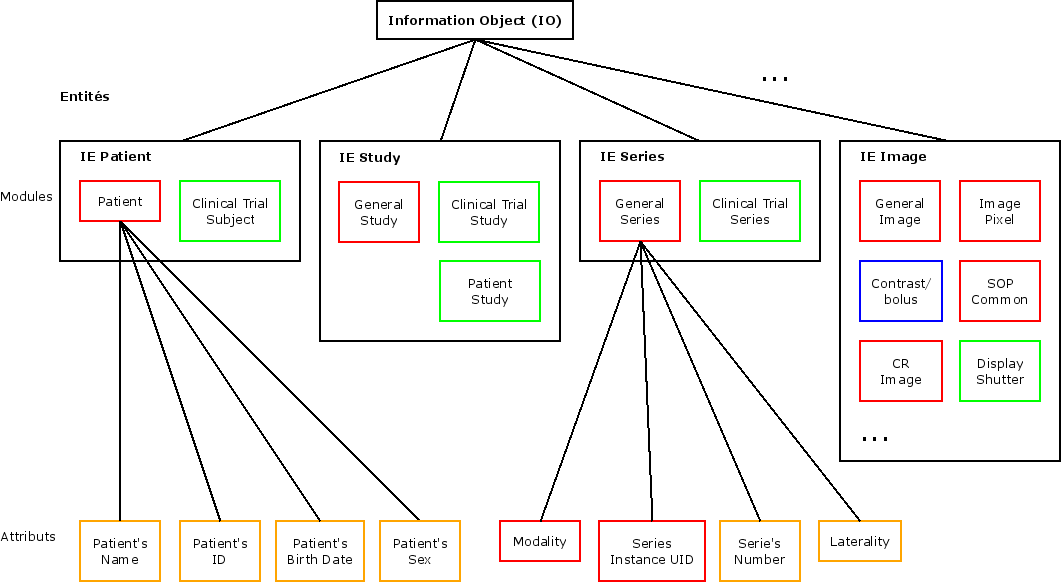
\includegraphics[width=\linewidth]{./figures/IO-definition.png}
	\end{center}
}

\frame
{
	\frametitle{Objet}
	\begin{itemize}
		\item<1-> Terminologie : objet = Data Set (\emph{e.g.} ensemble de donn\'ees).
		\item<2-> Un Data Set contient des Data Elements (ou \'el\'ements d'information).
		\item<3-> Chaque Data Element donne une valeur \`a un et un seul attribut de l'IOD.
		\item<4-> Contenu d'un Data Element :
		\begin{itemize}
			\item<5-> �tiquette d'identification (\emph{Tag}) contenant deux num\'eros.
			\item<6-> Type (\emph{VR} = \emph{Value Representation}).
			\item<7-> Taille en m\'emoire de la valeur.
			\item<8-> Valeur.
		\end{itemize}
		\item<9-> L'agr\'egation des Data Elements donnera un fichier DICOM.
	\end{itemize}
}

\frame
{
	\frametitle{Objet}
	
	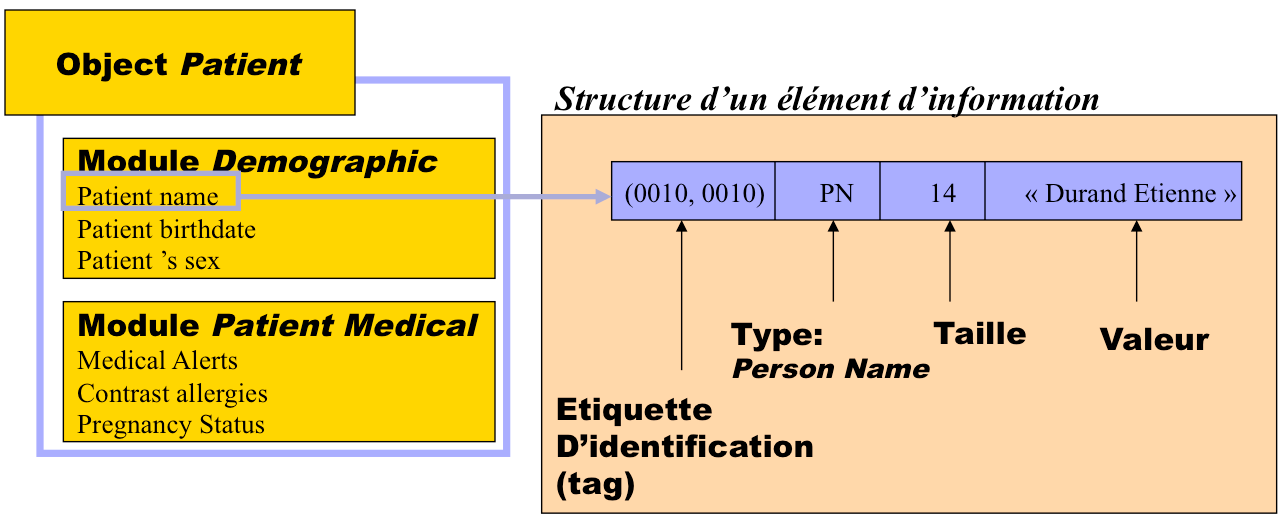
\includegraphics[width=\linewidth]{./figures/objet-dicom.png}
}

\frame
{
	\frametitle{Exemple d'objet : Examen (\emph{Study})}
	
	\begin{center}
		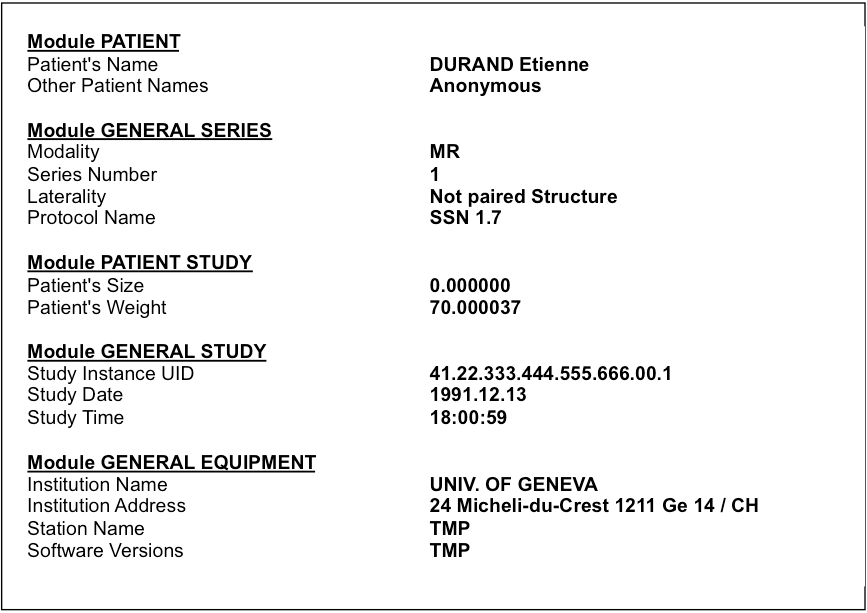
\includegraphics[width=.9\linewidth]{./figures/examen.png}
	\end{center}
}

\frame
{
	\frametitle{Exemple d'objet : Image IRM}
	
	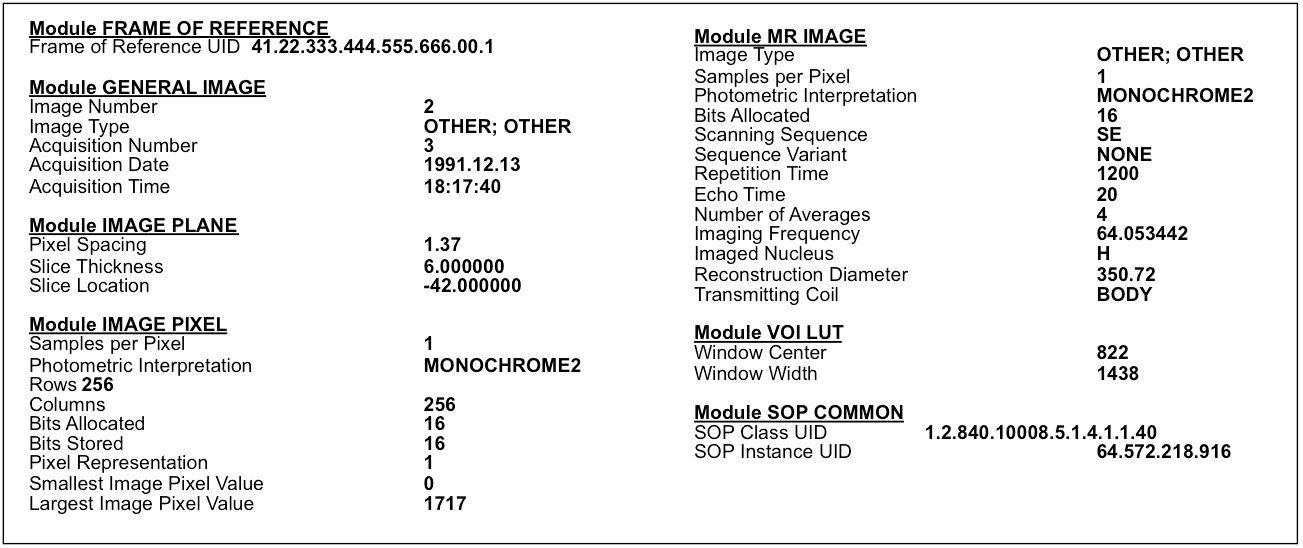
\includegraphics[width=\linewidth]{./figures/irm.png}
}


\section{Conclusions}

\frame
{
	\frametitle{Points forts}
	\begin{itemize}
		\item Norme compl\`ete et \'evolutive :
		\begin{itemize}
			\item<2-> Pas limit\'ee \`a la radiologie (oncologie, h\'ematologie, dermatologie, ophtalmologie, cardiologie, ORL,\ldots).
			\item<3-> Annotations sur les images, compression.
		\end{itemize}
		\item<4-> Libert\'e du choix d'achat d'\'equipement car ind\'ependance du fournisseur.
		\item<5-> Distribution d'images possible : support des protocoles de communication standards, TCP/IP notamment.
	\end{itemize}
}

\frame
{
	\frametitle{Points faibles}
	\begin{itemize}
		\item Complexe :
		\begin{itemize}
			\item<2-> Difficile \`a comprendre.
			\item<3-> Informatique de niche.
		\end{itemize}
		\item<4-> N\'ecessit\'e de patience : int\'egration progressive par les fournisseurs.
		\item<5-> P\'erim\`etre limit\'e : traite de la connectivit\'e, mais pas des fonctionnalit\'es des logiciels.
		\item<6-> Besoin d'un niveau de conformit\'e.
	\end{itemize}
}

\frame
{
	\frametitle{Pi\`eges et difficult\'es}
	\begin{itemize}
		\item Divergences/erreurs d'interpr\'etation de la norme.
		\item<2-> DICOM autorise le stockage d'informations sp\'ecifiques.
		\begin{itemize}
			\item<3-> Risque: faire du propri\'etaire sous le label DICOM
		\end{itemize}
		\item<4-> DICOM propose diff\'erentes alternatives pour d\'ecrire l'information.
		\begin{itemize}
			\item<5-> Annotations: 3 moyens de les transmettre.
		\end{itemize}
		\item<6-> Manque d'information disponible \`a l'installation sur l'activation des services DICOM.
	\end{itemize}
}

\frame
{
	\frametitle{Quelques contre-v\'erit\'es}
	\begin{itemize}
		\item "Je n'arrive plus \`a envoyer mes images. C'est \`a cause de DICOM !"
		\begin{description}
			\item<2->[Faux] DICOM utilise le r\'eseau, qui peut avoir ses d\'efaillances.
		\end{description}
		\item<3-> "DICOM d\'egrade la qualit\'e de mes images."
		\begin{description}
			\item<4->[Faux] DICOM n'invente rien : il repose sur des formats d'image qui peuvent ou non \^etres compress\'es.
		\end{description}
		\item<5-> "Ne vous inqui\'etez pas, je supporte enti\`erement DICOM"
		\begin{description}
			\item<6->[Faux] Remarque bien pr\'esomptueuse\ldots
			Possible, mais est-ce r\'ealiste ?
		\end{description}
	\end{itemize}
}

\frame
{
	\frametitle{Synth\`ese}
	\begin{itemize}
		\item<1-> Norme incontournable.
		\item<2-> Tr\`es largement et rapidement adopt\'ee par la majorit\'e des acteurs.
		\item<3-> Plus large couverture que l'imagerie radiologique
		\begin{itemize}
			\item<4-> Rapport structur\'e.
			\item<5-> Ouverture \`a toutes les imageries.
		\end{itemize}
		\item<6-> Norme \'evolutive.
	\end{itemize}
}

\section{Et si on a le temps�}

	\frame
	{
		\frametitle{Repr�sentations num�riques}
	}
	
	\frame
	{
		\frametitle{Pour le prochain cours}
		
		\begin{block}{Exercice}
			Jusqu'� combien pouvez-vous compter avec vos $10$ doigts ?
		\end{block}
		
		\onslide<2>
		{
			\begin{block}{Indice}
				Comptez en binaire�
			\end{block}
		}
	}
\section*{Annexes}

\frame
{
	\frametitle{UID}
	Unique Identifier
	\begin{itemize}
		\item 64 caract\`eres maximum, combinaison entre chiffres et points (OSI Object Identication, numeric form, ISO 8824)
		\item Afin d'en assurer l'unicit\'e, le UID est compos\'e par deux parties encha\^in\'ees :
		\begin{itemize}
			\item Une racine li\'ee \`a une organisation (racine attribu\'ee par la norme ISO 9823-3)
			\item Un suffixe garanti unique par l'organisation
		\end{itemize}
	\end{itemize}
	La racine $1.2.840.10008$ identifie le standard DICOM
}

\frame
{
	\frametitle{\'Etiquettes d'identification}
	\begin{itemize}
		\item S\'epar\'ees en Groupe et \'el\'ement
		\item Notation hexad\`ecimale (0123456789ABDCEF)
		\item Identification unique, typage li\'e
		\begin{description}
			\item[(0010,0010)] Patient Name (PN)
			\item[(0010,0020)] Patient ID (LO)
			\item[(0008,0050)] Accession Number (SH)
			\item[(0020,000d)] Study Instance UID (UI)
			\item[(7fe0,0010)] Pixel Data (OW ou OB)
		\end{description}
	\end{itemize}
}

%\frame
%{
%	\frametitle{Typage}
%	Diff\'erents types possibles pour les Data Elements.
%	Analogie avec le jeu des formes pour les enfants.
%}

\frame
{
	\frametitle{SOP -- Images}
	Selon la classe SOP, un objet DICOM peut d\'ecrire une ou plusieurs images.
	
	Par exemple, il est normal de stocker une s\'equence d'images pour une \'echographie.
	
	G\'en\'eralement, on parle d'Enhanced DICOM pour les objets d\'ecrivant plusieurs images.
}



%\section{Notions pr\'eliminaires}

	\frame
	{
		\frametitle{Qu'est-ce que DICOM ?}
		
		\begin{block}{\textbf{D}igital \textbf{I}maging and \textbf{Co}mmunications in \textbf{M}edicine}
		\begin{itemize}
			\item Digital = Num\'erique
		    	\item Imaging = Imagerie
		    	\item Communications
		    	\item Medicine
			\end{itemize}
		\end{block}
		
		\begin{block}{Vocabulaire}
		\begin{itemize}
			\item Modalit\'e
			\item RIS/PACS
			\item Instance
			\item UID = Unique Identifier
		\end{itemize}
		\end{block}
	}
	
	\frame
	{
		\frametitle{La norme en d\'etails}
		Plus de $5600$ pages de documentation r\'eparties en $18$ chapitres.
		
		\begin{columns}\begin{scriptsize}
	  	\begin{column}[t]{0.5\linewidth}
			\begin{itemize}
				\item DICOM Part 1: Introduction and Overview (34 pages)
				\item Part 2: Conformance (322 pages)
				\item Part 3: Information Object Definitions (1464 pages)
				\item Part 4: Service Class Specifications (422 pages)
				\item Part 5: Data Structures and Encoding (138 pages)
				\item Part 6: Data Dictionary (212 pages)
				\item Part 7: Message Exchange (128 pages)
				\item Part 8: Network Communication Support for Message Exchange (72 pages)
%				\item \st{DICOM Part 9: Point-to-Point Communication Support for Message Exchange}
				\item DICOM Part 10: Media Storage and File Format for Media Interchange (48 pages)
			\end{itemize}
	  	\end{column}
	  	\begin{column}[t]{0.5\linewidth}
			\begin{itemize}
				\item Part 11: Media Storage Application Profiles (96 pages)
				\item Part 12: Media Formats and Physical Media for Media Interchange (92 pages)
%				\item \st{DICOM Part 13: Print Management Point-to-Point Communication Support}
				\item Part 14: Grayscale Standard Display Function (66 pages)
				\item Part 15: Security and System Management Profiles (142 pages)
				\item Part 16: Content Mapping Resource (1242 pages)
				\item Part 17: Explanatory Information (786 pages)
				\item Part 18: Web Services (160 pages)
				\item Part 19: Application Hosting (96 pages)
				\item Part 20: Imaging Reports using HL7 Clinical Document Architecture (152 pages)
			\end{itemize}
	  	\end{column}\end{scriptsize}
	  	\end{columns}
	}


%\section{Histoire du DICOM}

	\frame
	{
		\frametitle{Pr\'ehistoire}
		
		\begin{itemize}
			\item Arriv\'ee du num\'erique en m\'edecine.
			\item Stockage, transmission, affichage des images : constructeur d\'ependant.
			\item Solutions propri\'etaires (par opposition \`a solutions ouvertes) :
			\begin{itemize}
				\item argument commercial : "Mon protocole est meilleur que les autres", "Nos produits ont une excellente interaction entre eux", "Nous g\'erons tout de A \`a Z" ;
				\item interaction impossible entre marques diff\'erentes.
			\end{itemize} 
			\item Cons\'equences :
			\begin{itemize}
				\item pi\`ege commercial : obligation d'acqu\'erir les stations d'acquisition et de traitement ad\'equates, et changer de marque peut rendre les anciens examens illisibles ;
				\item pi\`ege m\'edical : difficile de communiquer entre coll\`egues.
			\end{itemize}
		\end{itemize}
	}
					
	\frame
	{
		\frametitle{D\'ebuts du DICOM}
		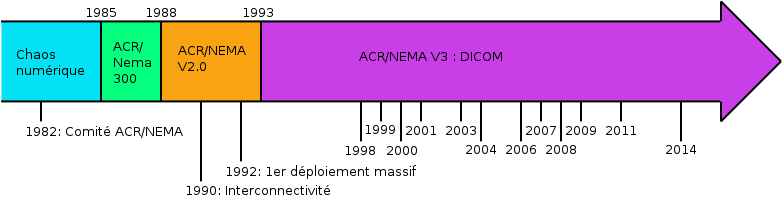
\includegraphics[width=\linewidth]{./figures/chrono-dicom.png}

		\begin{itemize}
			\item 1\up{\`ere} version ACR/NEMA 300 en 1985 : peu accept\'e car vague et contenant des incoh\'erences.
			\item 2\up{\`eme} version en 1988 : transmission des images par le connecteur mat\'eriel EIA-485, adopt\'e par quelques constructeurs.
			\item 3\up{\`eme} version en 1993 : ind\'ependance du connecteur, donc support TCP.
		\end{itemize}
	}
	
	\frame
	{
		\frametitle{Support / Sponsoring}
		\begin{itemize}
			\item ACR : American College of Radiology
			\item NEMA : National Electrical Manufacturers Association
			\item JIRA : Japan Investor Relations Association
			\item CEN : Comit\'e Europ\'een de Normalisation
			\item IEEE, HL7, ANSI,\ldots
		\end{itemize}
	}

	\frame
	{
		\frametitle{DICOM aujourd'hui}
		\begin{itemize}
			\item Standard accept\'e mondialement.
			\item Actuellement en version $2014$b : on parle des versions par leur ann\'ee (officiellement, toujours en version 3, ou PS3)
			\item Diversit\'e des \'equipements support\'es : RX, CT, IRM, US, PET, SPECT, Angio, ECG,\ldots
			\item Adopt\'e par de nombreux constructeurs : GE, Siemens, Philips, Toshiba,\ldots
		\end{itemize}
	}

%\section{Principes de DICOM}

	\subsection{Objectifs de DICOM}
	
	\frame
	{
		\frametitle{Buts g\'en\'eraux}
		\begin{itemize}
			\item Trouver un langage commun pour l'\'echange (images et donn\'ees pertinentes) entre \'equipements d'imagerie : mettre en place un standard.
			\item Pousser les vendeurs \`a parler et comprendre ce langage commun.
			\item Standardiser :
			\begin{itemize}
				\item le stockage (i.e. format de fichier) ;
				\item et la communication des donn\'es (i.e. protocoles de communication).
			\end{itemize}
		\end{itemize}
	}
	
	\frame
	{
		\frametitle{Buts sp\'ecifiques}
		
        Il faut que lors de l'installation d'une nouvelle modalit\'e, le DICOM permette, sans changement d'un quelconque composant logiciel (\emph{i.e.~Plug~\&~Play}) :
		\begin{itemize}
			\item l'interrogation du PACS ;
			\item la r\'ecup\'eration des images cr\'e\'ees par d'autres syst\`emes ;
			\item l'affichage des images ;
			\item et la production d'images lisibles par les syst\`emes d'autres constructeurs.
		\end{itemize}
	}

	\subsection{Fondements th\'eoriques}

	\frame
	{
		\frametitle{Prescription d'un examen radiologique}
		\begin{itemize}
			\item Sch\'ematisation de la proc\'edure :
			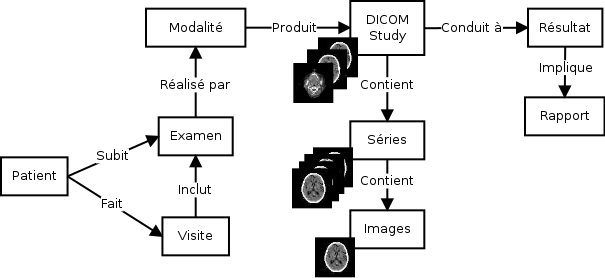
\includegraphics[width=\linewidth]{./figures/scenario.png}
			\item DICOM d\'ecrit ces donn\'ees et ces relations.
			\item La pr\'ecision du contenu et des liens d\'epend des outils et des utilisateurs (\emph{e.g.} RIS, PACS).
		\end{itemize}
	}

	\frame
	{
		\frametitle{Traduire le r\'eel en num\'erique}
		
		\begin{itemize}
			\item Un objet DICOM combine donc :
			\begin{itemize}
				\item des donn\'ees, ou informations (e.g. nom du patient, donn\'ees de l'image,\ldots) ;
				\item et services, ou fonctions (e.g. sauvegarder, imprimer,\ldots).
			\end{itemize}
			
			\item Le traitement DICOM d'une information consiste alors \`a regrouper :
			\begin{itemize}
				\item les donn\'ees, contenues dans un \emph{Information Objet}, que la norme d\'efinit gr\^ace \`a une \emph{Information Object Definition} (ou \emph{IOD}) ;
				\item et une fonction sp\'ecifique, ou \emph{Service}, d\'efinie par un \emph{DICOM Message Service Element} (ou \emph{DIMSE}).
			\end{itemize}
		\end{itemize}
	}
	
	\frame
	{
		\frametitle{SOP Class UID}

		\begin{itemize}
			\item La combinaison Information Objet + Service est :
			\begin{itemize}
				\item appel\'ee \emph{Service/Object Pair} (ou \emph{SOP}) ;
				\item un \'el\'ement important pour d\'eterminer la conformit\'e � la norme ;
				\item identifi\'ee par un identifiant unique nomm\'e \emph{SOP Class UID}.
			\end{itemize}
		
			\item Norme DICOM = annuaire de SOP.\\
			SOP Class UID = num\'ero unique pour trouver \`a quelle paire Service/Objet correspond un objet DICOM.
			\item Analogie : annuaire\\
			Une entr\'ee = paire \{t\'el\'ephone $+$ adresse\}.
			\item Exemples de SOP Class UID :
			\begin{description}
				\item[$1.2.840.10008.5.1.4.1.1.1$] CR Image Store (enregistrer un CR) ;
				\item[$1.2.840.10008.5.1.4.1.1.2$] CT Image Store (enregistrer un CT).
			\end{description}
		\end{itemize}
	}
	
	\frame
	{
		\frametitle{Sch\'ema de construction du SOP}
		\begin{center}
			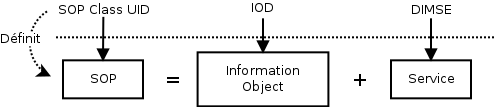
\includegraphics[width=\linewidth]{./figures/sop-definition.png}
		\end{center}		
	}


%\section{Objets DICOM}

\frame
{
 	\frametitle{Information Object Definition}
  	L'IOD d\'etermine les attributs d\'ecrivant un objet.
  	\begin{description}
    		\item[Normalized IOD]~\\
			Repr\'esente une entit\'e unique du monde r\'eel (patient, visite, examen, r\'esultat, interpr\'etation,\ldots).
			Rarement appliqu\'e en pratique : cause complexit\'e et perte de performance.
    		\item[Composite IOD]~\\
			Repr\'esente certains d\'etails de plusieurs objets du monde r\'eel et les relations entre ces objets (nom du patient, date de l'examen,\ldots)
		\item[Attributes]~\\
			Les attributs d'un IOD d\'ecrivent les propri\'et\'es d'un \'el\'ement (instance d'un objet) du monde r\'eel.
  	\end{description}
}

\frame
{
 	\frametitle{IOD composite}
 	\begin{itemize}
		\item IOD compos\'es d'\emph{Information Entities} ou \emph{IE}.
   		\item Une IE comporte un ou plusieurs \emph{Modules}.
		\begin{description}
			\item[Mandatory] Module obligatoire.
			\item[Conditinal] Module conditionnel (obligatoire selon certaines conditions).
			\item[User Option] Module optionnel.
		\end{description}
   		\item Les modules sont compos\'es d'attributs de diff\'erents types ;
		\begin{description}
			\item[1] Obligatoire.
			\item[2] Obligatoire - peut \^etre vide.
			\item[3] Optionnel.
			\item[<1/2>C] Conditionnel.
		\end{description}
 	\end{itemize}
	En pratique, un objet DICOM est presque toujours une instance d'un IOD composite.
}

\frame
{
	\frametitle{Exemple d'IOD : image CR}
	
	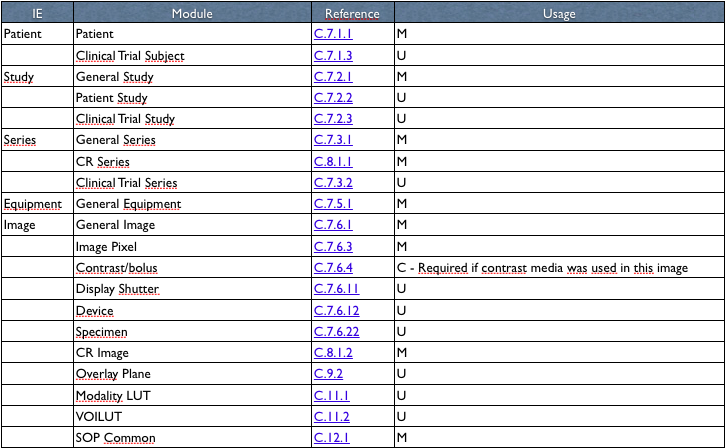
\includegraphics[width=\linewidth]{./figures/IOD-exemple.png}
}

\frame
{
	\frametitle{Objet}
	\begin{itemize}
		\item Terminologie : objet = Data Set
		\item Un Data Set est compos\'e de Data Elements.
		\item Chaque Data Element d\'ecrit un attribut de l'IOD.
		\item Data Element
		\begin{itemize}
			\item �tiquette d'identification (\emph{Tag}) contenant deux num\'eros.
			\item Type (\emph{VR} = \emph{Value Representation}).
			\item Taille de la valeur.
			\item Valeur.
		\end{itemize}
	\end{itemize}
}

\frame
{
	\frametitle{Objet}
	
	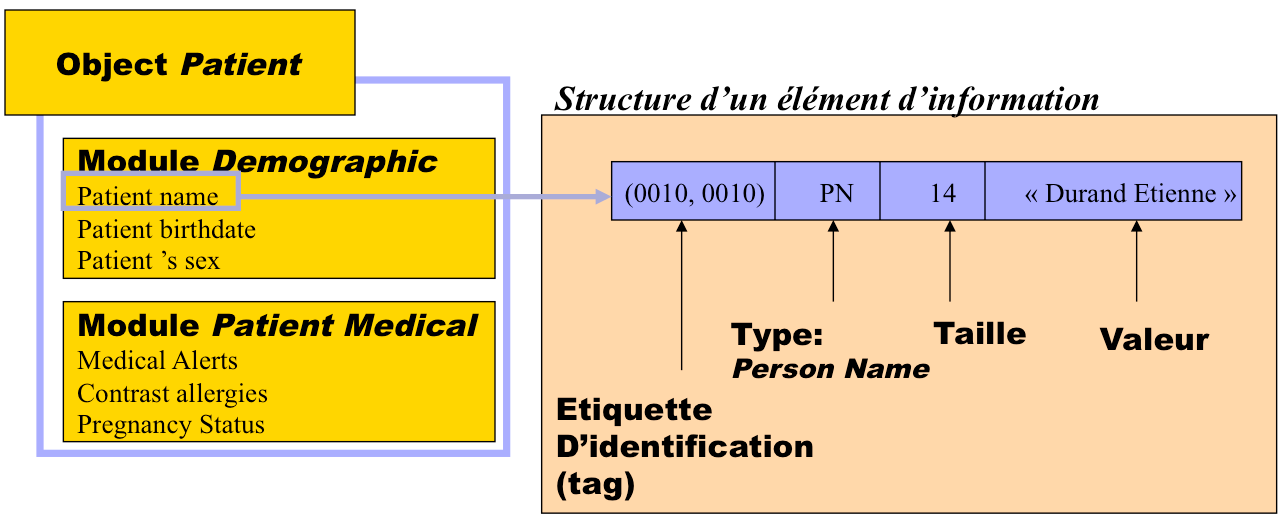
\includegraphics[width=\linewidth]{./figures/objet-dicom.png}
}

\frame
{
	\frametitle{Exemple d'objet : Examen (\emph{Study})}
	
	\begin{center}
		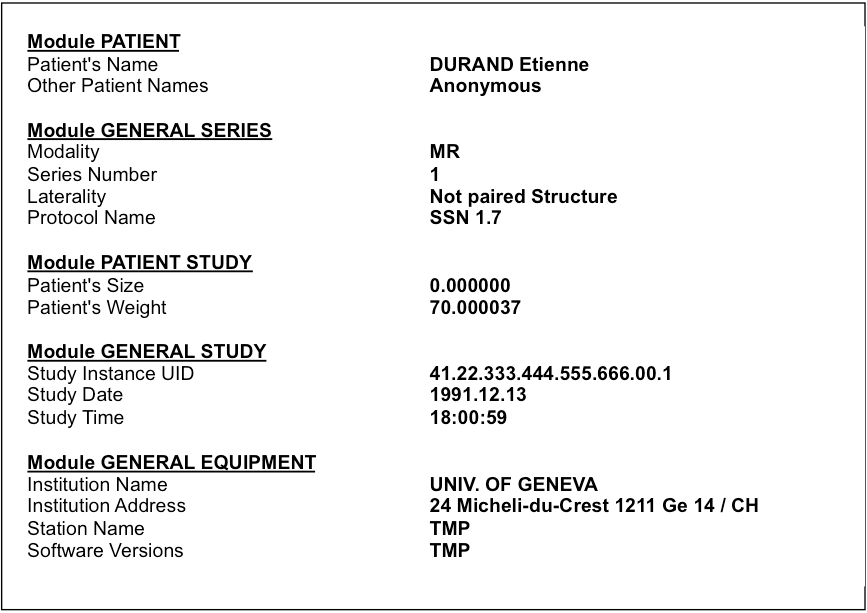
\includegraphics[width=.9\linewidth]{./figures/examen.png}
	\end{center}
}

\frame
{
	\frametitle{Exemple d'objet : Image IRM}
	
	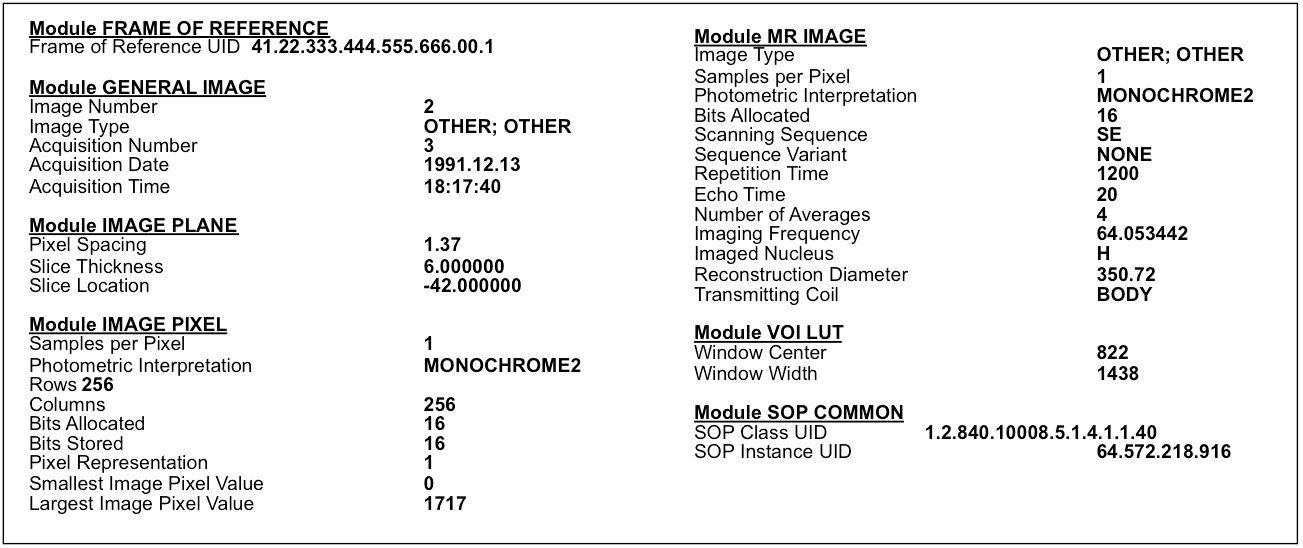
\includegraphics[width=\linewidth]{./figures/irm.png}
}

\frame
{
	\frametitle{Fichier DICOM}
	
	\begin{itemize}
		\item Encapsuler l'ensemble des objets dans un fichier.
		\begin{itemize}
			\item Ent\^ete : pr\'e-ent\^ete et objets.
			\item Image : donn\'ees brutes de l'image.
		\end{itemize}
		\item Les d\'etails au prochain cours.
	\end{itemize}
}

%\section{Conclusions}

\frame
{
	\frametitle{Points forts}
	\begin{itemize}
		\item Standard complet et \'evolutif :
		\begin{itemize}
			\item Pas limit\'e \`a la radiologie (oncologie, h\'ematologie, dermatologie, ophtalmologie, cardiologie, ORL,\ldots).
			\item Annotations sur les images, compression.
		\end{itemize}
		\item Libert\'e du choix d'achat d'\'equipement car ind\'ependance du fournisseur.
		\item Distribution d'images possible : support des protocoles de communication standards, TCP/IP notamment.
	\end{itemize}
}

\frame
{
	\frametitle{Points faibles}
	\begin{itemize}
		\item Complexe :
		\begin{itemize}
			\item Difficile \`a comprendre.
			\item Informatique de niche.
		\end{itemize}
		\item N\'ecessit\'e de patience : int\'egration progressive par les fournisseurs.
		\item P\'erim\`etre limit\'e : traite de la connectivit\'e, mais pas des fonctionnalit\'es des logiciels.
		\item Besoin d'un niveau de conformit\'e.
	\end{itemize}
}

\frame
{
	\frametitle{DICOM Conformance}
	\begin{itemize}
		\item Le standard pr\'evoit un document "DICOM Conformance Statement" dont le plan et la structure sont pr\'ed\'efinis.
		\item Par ce document, le fournisseur pr\'ecise le niveau de conformit\'e de son \'equipement \`a la norme DICOM.
		\begin{itemize}
			\item Applicable sur chaque mod\`ele, chaque version.
			\item Le document suit un plan pr\'evu dans la norme.
			\item Liste des SOP Class support\'ees et des r\^oles assur\'es (SCU, SCP).
		\end{itemize}
	\end{itemize}
}

\frame
{
	\frametitle{Pi\`eges et difficult\'es}
	\begin{itemize}
		\item Divergences/erreurs d'interpr\'etation de la norme.
		\item DICOM autorise le stockage d'informations sp\'ecifiques.
		\begin{itemize}
			\item Risque: faire du propri\'etaire sous le label DICOM
		\end{itemize}
		\item DICOM propose diff\'erentes alternatives pour d\'ecrire l'information.
		\begin{itemize}
			\item Annotations: 3 moyens de les transmettre.
		\end{itemize}
		\item Manque d'information disponible \`a l'installation sur l'activation des services DICOM.
	\end{itemize}
}

\frame
{
	\frametitle{Quelques contre-v\'erit\'es}
	\begin{itemize}
		\item "Je n'arrive plus \`a envoyer mes images. C'est \`a cause de DICOM !"
		\begin{description}
			\item[Faux] DICOM utilise le r\'eseau, qui peut avoir ses d\'efaillances.
		\end{description}
		\item "DICOM d\'egrade la qualit\'e de mes images."
		\begin{description}
			\item[Faux] DICOM n'invente rien : il repose sur des formats d'image qui peuvent ou non \^etres compress\'es.
		\end{description}
		\item "Ne vous inqui\'etez pas, je supporte enti\`erement DICOM"
		\begin{description}
			\item[Faux] Remarque bien pr\'esomptueuse?
			Possible, mais est-ce r\'ealiste ?
		\end{description}
	\end{itemize}
}

\frame
{
	\frametitle{Synth\`ese}
	\begin{itemize}
		\item Norme incontournable.
		\item Tr\`es largement et rapidement adopt\'ee par la majorit\'e des acteurs.
		\item Plus large couverture que l'imagerie radiologique
		\begin{itemize}
			\item Rapport structur\'e.
			\item Ouverture \`a toutes les imageries.
		\end{itemize}
		\item Norme \'evolutive.
	\end{itemize}
}


\end{document}
